\documentclass{article}
\usepackage{graphicx}
\usepackage{amsmath,amsthm,amssymb}
\usepackage[font=small,labelfont=bf]{caption}
\usepackage{tikz}
\usepackage{pgfplots}
\pgfplotsset{compat=1.18}
\usetikzlibrary{calc, angles, quotes, shapes.geometric, decorations.pathreplacing}
\usepackage{tkz-euclide}
\usepackage[inline]{asymptote}
\usepackage{float}
\usepackage[margin=1in]{geometry}
\usepackage{gensymb}
\usepackage[normalem]{ulem}
\usepackage{hyperref}
\hypersetup{
    colorlinks=true,
    linkcolor=blue,
    filecolor=magenta,      
    urlcolor=cyan,
    pdftitle={Overleaf Example},
    pdfpagemode=FullScreen,
    }
\usepackage{fancyhdr}
\pagestyle{fancy}
\fancyhead[R]{Enoch Yu}
\pagenumbering{gobble}
\usepackage{enumitem}
\newtheorem{theorem}{Theorem}[section]
\newtheorem{lemma}[theorem]{Lemma}
\newtheorem*{lemma*}{Lemma}
\newtheorem{sublemma}{Lemma}[section]
\newtheorem{proposition}{Proposition}
\newtheorem{corollary}{Corollary}[theorem]
\newtheorem{example}{Example}[section]
\newtheorem*{example*}{Example}
\newenvironment{solution}{\begin{trivlist}\item[]{\bf Solution}}{\qed \end{trivlist}}
\newcommand{\verteq}{\rotatebox{90}{$\;\;=\;\;$}}
\newcommand*\circled[1]{\tikz[baseline=(char.base)]{
            \node[shape=circle,draw,inner sep=1pt] (char) {#1};}}
\newcommand{\triangled}[1]{\tikz[baseline=(char.base)]{
            \node[shape=regular polygon, regular polygon sides=3, draw, inner sep=0.2pt] (char) {#1};}}

\title{Problem Set 34}
\author{Enoch Yu}
\date{July 2025}

\begin{document}

\section*{Problem}
A Circle $O$ of radius $r$ is inscribed to $\triangle{ABC}$ at $D$, $E$, and $F$. $\angle{C} = 60^\circ$. The length of the side opposite to $\angle{C}$ is $c = \sqrt{3}$. Find the range of $r$.
\begin{solution}
\begin{center}
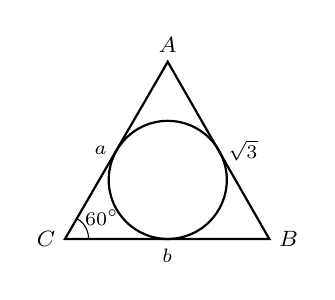
\begin{tikzpicture}[scale=1.5]
    \coordinate (A) at (0.87, 1.5);
    \coordinate (B) at (1.73, 0);
    \coordinate (C) at (0, 0);
    \coordinate (O) at (0.87, 0.5);

    \draw[thick] (A) -- (B) -- (C) -- cycle;
    \draw[thick] (O) circle (0.5);

    \node[above] at (A) {\footnotesize $A$};
    \node[right] at (B) {\footnotesize $B$};
    \node[left] at (C) {\footnotesize $C$};

    \node[left] at ($(A)!0.5!(C)$) {\scriptsize $a$};
    \node[right] at ($(A)!0.5!(B)$) {\scriptsize $\sqrt{3}$};
    \node[below] at ($(B)!0.5!(C)$) {\scriptsize $b$};

    \draw pic["\scriptsize $60^\circ$", draw=black, angle radius=0.3cm, angle eccentricity=1.8] {angle=B--C--A};
\end{tikzpicture}
\end{center}
From the diagram, notice that the values of $a + b$ and $ab$ could be written in terms of $r$.
\begin{align*}
    a - \tan60^\circ \cdot r + b - \tan60^\circ \cdot r &= \sqrt{3} \\
    a + b &= \sqrt{3}(2r + 1) \\
    \frac{r(a + b + \sqrt{3})}{2} &= \frac{\sqrt{3}ab}{4} \\
    \frac{r\left( \sqrt{3}(2r + 1) + \sqrt{3} \right)}{2} &= \frac{\sqrt{3}ab}{4} \\
    ab &= 2r(2r + 2)
\end{align*}
Let $a$ and $b$ be the root of the equation
\[
t^2 - \sqrt{3}(2r + 1) + 4r^2 + 4r = 0
\]
Discriminant could be used since $a$ and $b$ are positive numbers.
\begin{align*}
    12r^2 + 12r + 3 - 16r^2 - 16r &\geq 0 \\
    4r^2 + 4r - 3 &\leq 0 \\
    (2r + 3)(2r - 1) &\leq 0 \\
    \therefore \boxed{0 < r \leq \frac{1}{2}}
\end{align*}
\end{solution}

\section*{Problem}
Show that there is one and only one of real numbers $x$, $y$, and $z$ that is at least $\sqrt[3]{4}$ if $x + y + z = 0$ and $xyz = 1$.
\begin{proof}
WLOG, let $x \leq y < z$ and let $x$ and $y$ be the solution to the following equation.
\[
t^2 + zt + \frac{1}{z} = 0
\]
Using discriminant, $z^2 - \frac{4}{z} \geq 0$. Because $z$ must be a positive number, $z^3 \geq 4$. In other words, only $z \geq \sqrt[3]{4}$.
\end{proof}

\section*{Problem}
Show that $1 < a + b < \frac{4}{3}$ and $\frac{8}{9} < a^2 + b^2 < 1$ if $a + b + c = a^2 + b^2 + c^2 = 1$, and $a > b > c$.
\begin{proof}
Let $x = a - c$ and $y = b - c$. Therefore, $x > y$. Moreover, the following equations are true.
\begin{align*}
    x + y
    &= a + b - 2c \\
    &= 1 - 3c \\
    xy
    &= (a - c)(b - c) \\
    &= ab - c(a + b) + c^2 \\
    &= -2c(a + b) + c^2 \\
    &= -2c(1 - c) + c^2
\end{align*}
Let $x$ and $y$ be the solution for the following equation.
\[
t^2 - (1 - 3c)t - 2c(1 - c) + c^2 = 0
\]
Therefore, the following conditions must satisfy.
\[
\begin{cases}
    1 - 3c > 0 \\
    - 2c(1 - c) + c^2 > 0 \\
    (1 - 3c)^2 + 8c(1 - c) - 4c^2 > 0
\end{cases}
\]
Therefore, $c < \frac{1}{3}$, $c < 0$ or $c > \frac{2}{3}$, and $-\frac{1}{3} < c < 1$. In other words, $-\frac{1}{3} < c < 0$. \\
\begin{minipage}[t]{0.5\textwidth}
\begin{align*}
    -\frac{1}{3} &< 1 - a - b < 0 \\
    \therefore 1 &< a + b < \frac{4}{3}
\end{align*}
\end{minipage}
\begin{minipage}[t]{0.5\textwidth}
\begin{align*}
    0 &< c^2 < \frac{1}{9} \\
    0 &< 1 - a^2 - b^2 < \frac{1}{9} \\
    \therefore \frac{8}{9} &< a^2 + b^2 < 1
\end{align*}
\end{minipage}
\end{proof}

\section*{Problem}
Find the range of the function $y = \sqrt{2 - x} + \sqrt{x - 1}$.
\\\\
\textbf{Solution I}
Let $a = \sqrt{2 - x}$ and $b = \sqrt{x - 1}$. Therefore, $a + b = y$ and $(a + b)^2 = 1 + 2\sqrt{(2 - x)(x - 1)} = y^2$. In other words, $ab = \frac{y^2 - 1}{2}$.
Let $a$ and $b$ be the roots of the equation $t^2 - yt + \frac{y^2 - 1}{2} = 0$. Using discriminant, $y^2 - 2y^2 + 2 \geq 0$, or $-\sqrt{2} \leq y \leq \sqrt{2}$. However, notice that $y > 0$ and $y \leq -1$ or $y \geq 1$. Therefore, the range for $y$ is $\boxed{[-1, 1]}$.
\qed
\\\\
\textbf{Solution II}
First, notice that $1 \leq x \leq 2$. Moreover, the function is a polynomial. Therefore, the following equations are true.
\begin{align*}
    y' &= \frac{-1}{\sqrt{2 - x}} + \frac{1}{\sqrt{x - 1}} \\
    y'' &= \frac{-1}{2\sqrt{(2 - x)^3}} - \frac{1}{\sqrt{(x - 1)^3}} < 0
\end{align*}
In other words, $y$ is a concave down function that has a critical point at $x = 1.5$. Therefore, the minimum value of $y$ is $1$ and the maximum is $\sqrt{2}$. Thus, $\boxed{1 \leq y \leq \sqrt{2}}$.
\qed

\section*{Problem}
How many distinct ordered triples $(x, y, z)$ satisfy the following equations?
\begin{align*}
    x + 2y + 4z &= 12 \\
    xy + 4yz + 2xz &= 22 \\
    xyz &= 6
\end{align*}
\begin{solution}
First and foremost, notice that the problem might have been more affable if the coefficients of the variables in the second equation were different. If a pattern is found, any equation could be forcibly changed for the pattern to satisfy flawlessly.
\begin{align*}
    x + 2y + 4z &= 12 \\
    2xy + 8yz + 4xz &= 44 \\
    8xyz &= 48
\end{align*}
Let $a = x$, $b = 2y$, and $c = 4z$. Then, the following equations are true.
\begin{align*}
    a + b + c &= 12 \\
    ab + bc + ca &= 44 \\
    abc &= 48
\end{align*}
Using, Vieta's formula, it is evident that $a$, $b$, and $c$ are the real roots of the following equation.
\[
t^3 - 12t^2 + 44t - 48 = 0
\]
Solving for $t$ will lead to the values of $a$, $b$, and $c$.
\begin{align*}
    t^3 - 12t^2 + 44t - 48 &= 0 \\
    (t - 2)(t - 4)(t - 6) &= 0 \\
    t = 2, 4, 6
\end{align*}
Because $2, 4, 6$ are all different numbers, there exists $3!$, or $\boxed{6}$, distinct ordered triples $(x, y, z)$.
\end{solution}

\section*{Problem}
Find all pairs of integers $(a, b)$ such that the polynomial $ax^{17} + bx^{16} + 1$ is divisible by $x^2 - x - 1$.
\\\\
\textbf{Solution I}
Notice that the coefficients for $x^{15}$ to $x$ are all zero for the polynomial. Therefore, the polynomial could intuitively be factored.
\[
(x^2 - x - 1)(\uwave{\qquad\qquad\qquad\qquad} + x - 1)
\]
Notice that a Fibonacci sequence with alternating signs must appear for the coefficients of $x^i$. Notice that $F_{15} = 987$ and $F_{14} = 610$. Therefore, the pair of integer is $\boxed{(987, -1597)}$.
\qed
\\\\
\textbf{Solution II}
Let $\alpha$ and $\beta$ be the roots of the divisor. Notice that $\alpha$ and $\beta$ are also the roots of the first polynomial. Therefore, the following equations are true.
\begin{align*}
    a\alpha^{17} + b\alpha^{16} &= -1 \\
    a\alpha^{17}\beta^{16} + b\alpha^{16}\beta^{16} &= -\beta^{16} \\
    a\beta^{17}\alpha^{16} + b\alpha^{16}\beta^{16} &= -\alpha^{16} \\
    a\alpha + b &= -\beta^{16} \\
    a\beta + b &= -\alpha^{16}
\end{align*}
Therefore, $a(\alpha - \beta) = \alpha^{16} - \beta^{16} = (\alpha^8 + \beta^8)(\alpha^4 + \beta^4)(\alpha^2 + \beta^2)(\alpha + \beta) = 987$. Moreover, $b = -1597$. Thus, the ordered pair is $\boxed{(987, -1597)}$.

\end{document}
